\documentclass[12pt]{article}

\usepackage{sbc-template}
\usepackage[brazil]{babel}
\usepackage[utf8]{inputenc}
\usepackage{graphicx}
\usepackage{booktabs}
\usepackage{amsmath}
\usepackage{url}
\usepackage{hyperref}
\usepackage{float}

% -----------------------------------------------------------------------
% Certifique-se de que o arquivo sbc-template.sty está no mesmo diretório
% no Overleaf (extraído do ZIP SBC_Conferences_Template).
% As imagens também devem ser enviadas ao Overleaf:
%   resumo_ordenacao.png, ord_comparacoes.png, ord_tempos.png,
%   ord_trocas.png, busca_comparacoes.png, busca_tempo.png
% -----------------------------------------------------------------------

\sloppy

\title{Análise de Algoritmos de Ordenação e Busca Aplicados a uma Base de Dados Biomédica da Coluna Vertebral}

\author{[Nome do Aluno 1]\inst{1}, [Nome do Aluno 2]\inst{1}, [Nome do Aluno 3]\inst{1}}

\address{Universidade Tecnológica Federal do Paraná (UTFPR) \\
  Campus Medianeira\\
  Medianeira -- PR -- Brasil
  \email{\{aluno1, aluno2, aluno3\}@alunos.utfpr.edu.br}
}

\begin{document}

\maketitle

% -----------------------------------------------------------------------
\begin{abstract}
This paper presents a comparative analysis of sorting and searching algorithms applied to a real biomedical dataset. The dataset, sourced from the UCI Machine Learning Repository, contains 310 records of orthopedic patients classified as Normal or Abnormal based on six biomechanical attributes of the lumbar spine. Six sorting algorithms were implemented and evaluated in C++: Bubble Sort (with optimization flag), Insertion Sort, Selection Sort, Shell Sort, Quick Sort Lomuto, and Quick Sort Hoare. Three input scenarios were tested: unsorted, sorted ascending, and sorted descending data. Sequential and binary search algorithms were also compared before and after sorting. Results confirm that divide-and-conquer algorithms (Shell Sort and Quick Sort variants) significantly outperform quadratic algorithms, and that binary search achieves a search in as few as 8--9 comparisons against up to 310 for sequential search in the worst case.
\end{abstract}

\begin{resumo}
Este artigo apresenta uma análise comparativa de algoritmos de ordenação e busca aplicados a um dataset biomédico real. A base de dados, proveniente do UCI Machine Learning Repository, contém 310 registros de pacientes ortopédicos classificados como Normal ou Anormal com base em seis atributos biomecânicos da coluna lombar. Seis algoritmos de ordenação foram implementados e avaliados em C++: Bubble Sort (com flag de otimização), Insertion Sort, Selection Sort, Shell Sort, Quick Sort Lomuto e Quick Sort Hoare. Três cenários de entrada foram testados: dados desordenados, ordenados em ordem crescente e ordenados em ordem decrescente. Os algoritmos de busca sequencial e binária também foram comparados antes e após a ordenação. Os resultados confirmam que algoritmos de divisão e conquista (Shell Sort e variantes do Quick Sort) superam significativamente os algoritmos quadráticos, e que a busca binária localiza um elemento em apenas 8--9 comparações contra até 310 da busca sequencial no pior caso.
\end{resumo}

% -----------------------------------------------------------------------
\section{Introdução}

O tempo de recuperação de informações em um sistema computacional está diretamente vinculado à qualidade dos algoritmos que organizam e percorrem os dados armazenados. Em sistemas do mundo real --- sejam eles catálogos de e-commerce, registros hospitalares ou sistemas de diagnóstico médico --- a eficiência algorítmica impacta diretamente a experiência do usuário e a confiabilidade dos resultados \cite{ziviani2005}.

Neste contexto, este trabalho investiga o comportamento prático de seis algoritmos de ordenação e dois algoritmos de busca aplicados a uma base de dados biomédica real. O dataset escolhido é o \textit{Column 2C Weka Dataset}, disponibilizado pelo UCI Machine Learning Repository, que reúne medições biomecânicas da coluna vertebral de pacientes ortopédicos. Cada registro é caracterizado por seis atributos numéricos contínuos --- incidência pélvica, inclinação pélvica, ângulo de lordose lombar, inclinação sacral, raio pélvico e grau de espondilolistese --- além de uma classe diagnóstica binária (\textit{Normal} ou \textit{Abnormal}).

A escolha deste domínio justifica-se pela relevância prática: sistemas de apoio à decisão médica precisam ordenar e recuperar registros de pacientes com eficiência. Um sistema de triagem que leva segundos a mais para localizar um prontuário, em escala hospitalar, representa um custo significativo. A questão central investigada é: \textit{qual combinação de algoritmo de ordenação e estratégia de busca oferece o melhor desempenho neste conjunto de dados?}

O restante deste artigo está organizado da seguinte forma: a Seção~\ref{sec:fundamentacao} apresenta a fundamentação teórica dos algoritmos; a Seção~\ref{sec:metodologia} descreve o ambiente de testes e a metodologia de coleta de dados; a Seção~\ref{sec:resultados} expõe os resultados obtidos com tabelas e gráficos; a Seção~\ref{sec:analise} discute criticamente os resultados; e a Seção~\ref{sec:conclusao} apresenta as conclusões e recomendações.

% -----------------------------------------------------------------------
\section{Fundamentação Teórica}
\label{sec:fundamentacao}

\subsection{Algoritmos de Ordenação}

Algoritmos de ordenação reorganizam os elementos de uma estrutura segundo um critério de comparação. Sua análise considera três métricas principais: tempo de execução, número de comparações e número de trocas (movimentações físicas na memória) \cite{cormen2002}.

\textbf{Bubble Sort} percorre repetidamente o vetor, comparando pares adjacentes e trocando-os quando necessário. A versão com \textit{flag} de parada interrompe a execução caso nenhuma troca ocorra em uma passagem, obtendo complexidade $O(n)$ no melhor caso (vetor já ordenado) e $O(n^2)$ nos demais \cite{ziviani2005}.

\textbf{Insertion Sort} mantém uma sublista ordenada à esquerda e insere cada novo elemento na posição correta, deslocando os maiores. Sua complexidade é $O(n)$ no melhor caso e $O(n^2)$ no pior, sendo eficiente para dados quase ordenados \cite{ziviani2005}.

\textbf{Selection Sort} localiza o menor elemento do subvetor não ordenado e o posiciona na frente. Realiza exatamente $\frac{n(n-1)}{2}$ comparações independentemente da entrada, com complexidade $O(n^2)$ em todos os casos, porém com número mínimo de trocas: no máximo $n-1$ \cite{cormen2002}.

\textbf{Shell Sort} é uma generalização do Insertion Sort que permite trocas de elementos distantes, reduzindo o número total de movimentações. Utiliza uma sequência de incrementos decrescentes (\textit{gaps}). Sua complexidade depende da sequência de gaps; com a sequência de Knuth, obtém-se aproximadamente $O(n^{1,5})$ \cite{sedgewick1996}.

\textbf{Quick Sort} particiona o vetor em torno de um pivô e aplica o processo recursivamente. A variante \textbf{Lomuto} utiliza o último elemento como pivô, enquanto a variante \textbf{Hoare} usa dois ponteiros convergentes. No caso médio, ambas atingem $O(n \log n)$; no pior caso (pivô sempre extremo), $O(n^2)$ \cite{cormen2002}.

\subsection{Algoritmos de Busca}

\textbf{Busca Sequencial} percorre os elementos um a um até encontrar o alvo ou exaurir a lista. Funciona em dados não ordenados, com complexidade $O(1)$ no melhor caso, $O(n/2)$ no caso médio e $O(n)$ no pior caso \cite{ziviani2005}.

\textbf{Busca Binária} requer dados previamente ordenados e divide o espaço de busca pela metade a cada iteração, descartando a metade onde o elemento não pode estar. Sua complexidade é $O(\log_2 n)$, tornando-a drasticamente mais eficiente que a busca sequencial para coleções de médio e grande porte \cite{cormen2002}.

% -----------------------------------------------------------------------
\section{Metodologia}
\label{sec:metodologia}

\subsection{Dataset}

O dataset utilizado é o \textit{Vertebral Column Data Set} (Column\_2C\_weka), disponível no UCI Machine Learning Repository \cite{uci_spine}. O arquivo \texttt{Dataset\_spine.csv} contém \textbf{310 registros} de pacientes ortopédicos e \textbf{7 colunas}: seis atributos biomecânicos numéricos de precisão dupla e uma classe diagnóstica categórica binária (\textit{Normal} ou \textit{Abnormal}). A distribuição das classes é de 210 registros Abnormal (67,7\%) e 100 registros Normal (32,3\%).

Os seis atributos são: \textit{pelvic incidence} (incidência pélvica), \textit{pelvic tilt} (inclinação pélvica), \textit{lumbar lordosis angle} (ângulo de lordose lombar), \textit{sacral slope} (inclinação sacral), \textit{pelvic radius} (raio pélvico) e \textit{grade of spondylolisthesis} (grau de espondilolistese). A ordenação foi aplicada sobre o campo \textbf{\textit{pelvic incidence}}, o atributo principal de caracterização biomecânica da pelve.

\subsection{Ambiente de Testes}

O sistema foi implementado em \textbf{C++17}, compilado com \texttt{g++ -O0} (sem otimizações do compilador) para medir o custo real dos algoritmos. O ambiente de testes é descrito na Tabela~\ref{tab:ambiente}.

\begin{table}[H]
\centering
\caption{Configuração do ambiente de testes.}
\label{tab:ambiente}
\begin{tabular}{ll}
\toprule
\textbf{Componente} & \textbf{Especificação} \\
\midrule
Processador & [Descreva seu processador, ex: Intel Core i5-10th Gen] \\
Memória RAM & [Ex: 8 GB DDR4 3200 MHz] \\
Sistema Operacional & [Ex: Ubuntu 22.04 / Windows 11] \\
Compilador & g++ 11.x, padrão C++17 \\
Flags de compilação & \texttt{-O0 -std=c++17} \\
\bottomrule
\end{tabular}
\end{table}

\subsection{Estrutura de Dados e Implementação}

Os dados do arquivo CSV foram lidos e armazenados em um \texttt{std::vector<Registro>}, onde \texttt{Registro} é uma \texttt{struct} com os seis atributos numéricos (\texttt{double}) e a classe diagnóstica (\texttt{std::string}).

Para cada algoritmo de ordenação foram instrumentados três contadores: \textbf{tempo de CPU} (medido com \texttt{clock()}), \textbf{número de comparações} e \textbf{número de trocas/movimentações}. Os algoritmos foram testados em três cenários de entrada distintos, conforme a Tabela~\ref{tab:cenarios}.

\begin{table}[H]
\centering
\caption{Cenários de entrada para os testes de ordenação.}
\label{tab:cenarios}
\begin{tabular}{ll}
\toprule
\textbf{Cenário} & \textbf{Descrição} \\
\midrule
Desordenado $\rightarrow$ Crescente & Dados na ordem original do CSV \\
Ordenado Crescente $\rightarrow$ Crescente & Dados já ordenados (melhor caso) \\
Decrescente $\rightarrow$ Crescente & Dados em ordem inversa (pior caso para alguns) \\
\bottomrule
\end{tabular}
\end{table}

Para os testes de busca, três alvos foram selecionados de forma a representar os casos melhor, médio e pior: o valor \textbf{63027} (posição próxima ao início no vetor desordenado --- melhor caso), \textbf{66804} (posição intermediária --- caso médio) e \textbf{33841} (posição próxima ao final no vetor desordenado --- pior caso). As buscas foram realizadas sobre o campo numérico \textit{pelvic incidence} multiplicado por $10^3$ e convertido para inteiro.

% -----------------------------------------------------------------------
\section{Resultados e Discussão}
\label{sec:resultados}

\subsection{Visão Geral dos Algoritmos de Ordenação}

A Figura~\ref{fig:resumo_ord} apresenta uma visão panorâmica dos três cenários de entrada, exibindo simultaneamente as curvas de comparações, trocas e tempo de execução para todos os algoritmos. É possível observar os cruzamentos de desempenho entre os algoritmos conforme o estado inicial dos dados muda --- em especial a inversão do Quick Sort Lomuto ao passar do cenário desordenado para o já ordenado.

\begin{figure}[H]
  \centering
  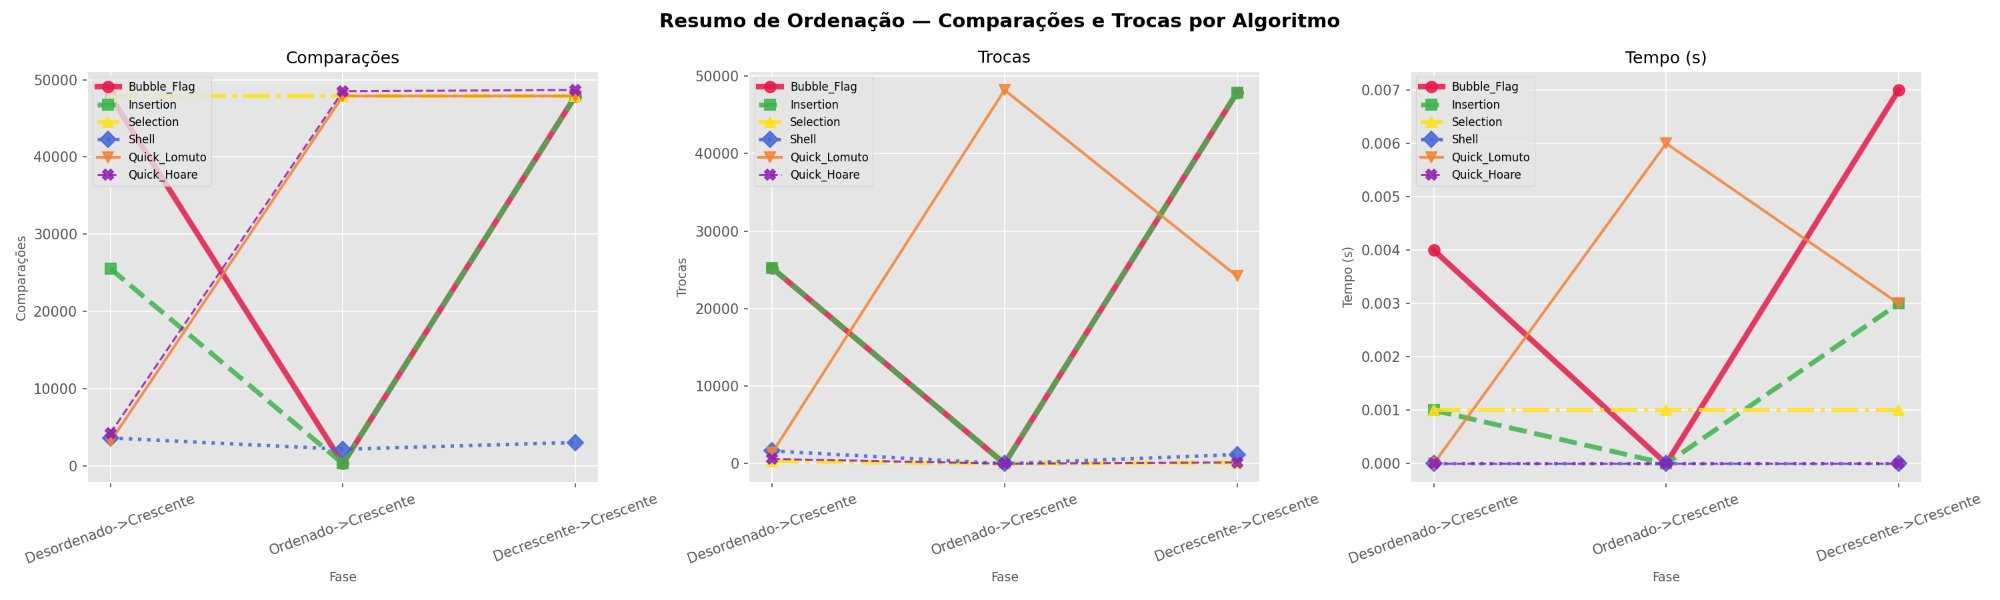
\includegraphics[width=\textwidth]{resumo_ordenacao.png}
  \caption{Resumo geral de ordenação: comparações, trocas e tempo por algoritmo nos três cenários.}
  \label{fig:resumo_ord}
\end{figure}

\subsection{Comparações por Algoritmo e Cenário}

A Figura~\ref{fig:ord_comp} detalha o número de comparações para cada algoritmo em cada um dos três cenários. Destaca-se a degradação do Quick Sort Lomuto na entrada já ordenada, que passa de 3.174 comparações no cenário desordenado para 47.895 --- equivalente ao Selection Sort.

\begin{figure}[H]
  \centering
  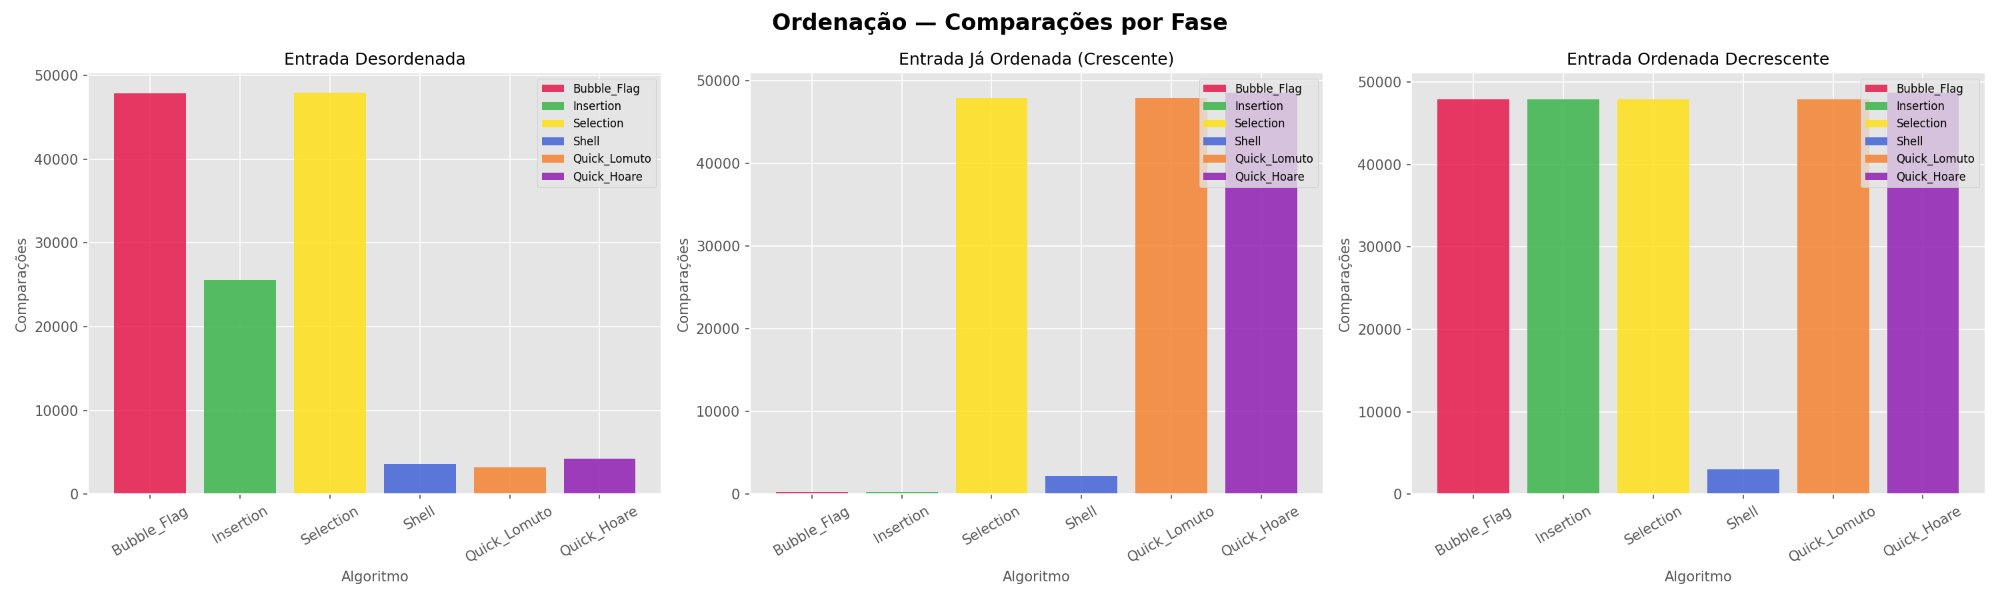
\includegraphics[width=\textwidth]{ord_comparacoes.png}
  \caption{Número de comparações por algoritmo nos três cenários de entrada (310 registros).}
  \label{fig:ord_comp}
\end{figure}

A Tabela~\ref{tab:ord_desordenado} sintetiza numericamente os resultados do cenário desordenado, o mais representativo de um ambiente de produção.

\begin{table}[H]
\centering
\caption{Ordenação a partir de dados desordenados (310 registros).}
\label{tab:ord_desordenado}
\begin{tabular}{lrrrl}
\toprule
\textbf{Algoritmo} & \textbf{Tempo (s)} & \textbf{Comparações} & \textbf{Trocas} & \textbf{Complexidade} \\
\midrule
Bubble Sort (Flag) & 0,004000 & 47.859 & 25.242 & $O(n^2)$ \\
Insertion Sort     & 0,001000 & 25.547 & 25.242 & $O(n^2)$ \\
Selection Sort     & 0,001000 & 47.895 &    306 & $O(n^2)$ \\
Shell Sort         & 0,000000 &  3.639 &  1.640 & $O(n^{1,5})$ \\
Quick Sort Lomuto  & 0,000000 &  3.174 &  1.380 & $O(n \log n)$ \\
Quick Sort Hoare   & 0,000000 &  4.245 &    606 & $O(n \log n)$ \\
\bottomrule
\end{tabular}
\end{table}

\begin{table}[H]
\centering
\caption{Ordenação a partir de dados já ordenados em ordem crescente (310 registros).}
\label{tab:ord_ordenado}
\begin{tabular}{lrrr}
\toprule
\textbf{Algoritmo} & \textbf{Tempo (s)} & \textbf{Comparações} & \textbf{Trocas} \\
\midrule
Bubble Sort (Flag) & 0,000000 &    309 &      0 \\
Insertion Sort     & 0,000000 &    309 &      0 \\
Selection Sort     & 0,001000 & 47.895 &      0 \\
Shell Sort         & 0,000000 &  2.175 &      0 \\
Quick Sort Lomuto  & 0,006000 & 47.895 & 48.204 \\
Quick Sort Hoare   & 0,000000 & 48.513 &      0 \\
\bottomrule
\end{tabular}
\end{table}

\begin{table}[H]
\centering
\caption{Ordenação a partir de dados em ordem decrescente (pior caso para vários algoritmos, 310 registros).}
\label{tab:ord_decrescente}
\begin{tabular}{lrrr}
\toprule
\textbf{Algoritmo} & \textbf{Tempo (s)} & \textbf{Comparações} & \textbf{Trocas} \\
\midrule
Bubble Sort (Flag) & 0,007000 & 47.895 & 47.895 \\
Insertion Sort     & 0,003000 & 47.895 & 47.895 \\
Selection Sort     & 0,001000 & 47.895 &    155 \\
Shell Sort         & 0,000000 &  3.053 &  1.177 \\
Quick Sort Lomuto  & 0,003000 & 47.895 & 24.179 \\
Quick Sort Hoare   & 0,000000 & 48.668 &    155 \\
\bottomrule
\end{tabular}
\end{table}

\subsection{Trocas por Algoritmo e Cenário}

A Figura~\ref{fig:ord_trocas} evidencia o comportamento atípico do Quick Sort Lomuto na entrada já ordenada: enquanto todos os demais algoritmos realizam zero trocas nesse cenário, o Lomuto executa 48.204 movimentações --- consequência direta da degeneração de sua estratégia de particionamento.

\begin{figure}[H]
  \centering
  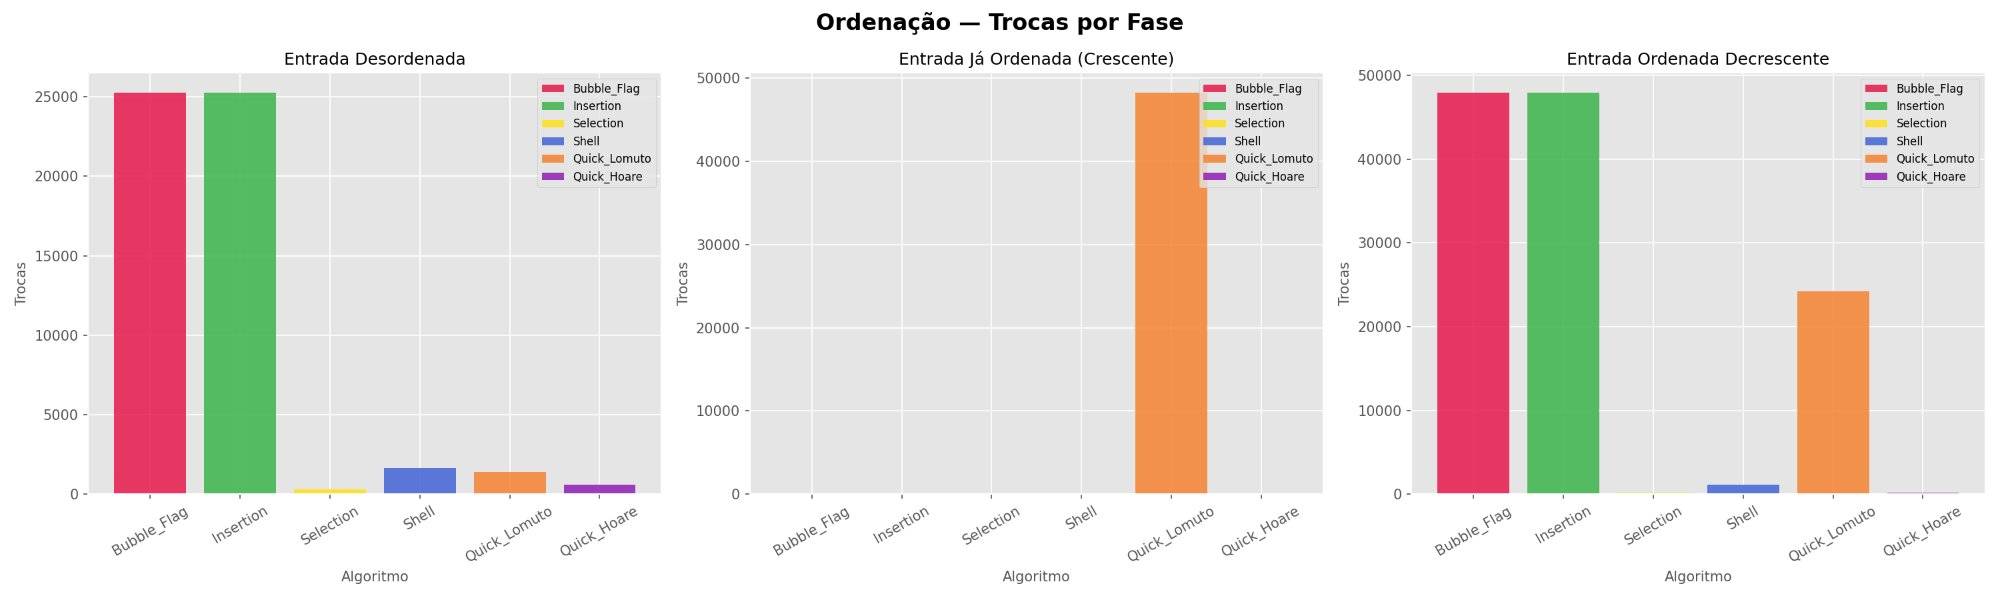
\includegraphics[width=\textwidth]{ord_trocas.png}
  \caption{Número de trocas/movimentações por algoritmo nos três cenários de entrada (310 registros).}
  \label{fig:ord_trocas}
\end{figure}

\subsection{Tempo de Execução por Algoritmo e Cenário}

A Figura~\ref{fig:ord_tempo} apresenta o tempo de CPU em segundos. A granularidade do relógio (\texttt{clock()}) limita a resolução a múltiplos de 1~ms, razão pela qual Shell Sort, Quick Sort Hoare e outros registram 0,000000~s --- abaixo do limiar de detecção. Ainda assim, o Bubble Sort se destaca como o mais lento no cenário desordenado (0,004~s) e no decrescente (0,007~s), enquanto o Quick Sort Lomuto apresenta o pico anômalo de 0,006~s na entrada já ordenada.

\begin{figure}[H]
  \centering
  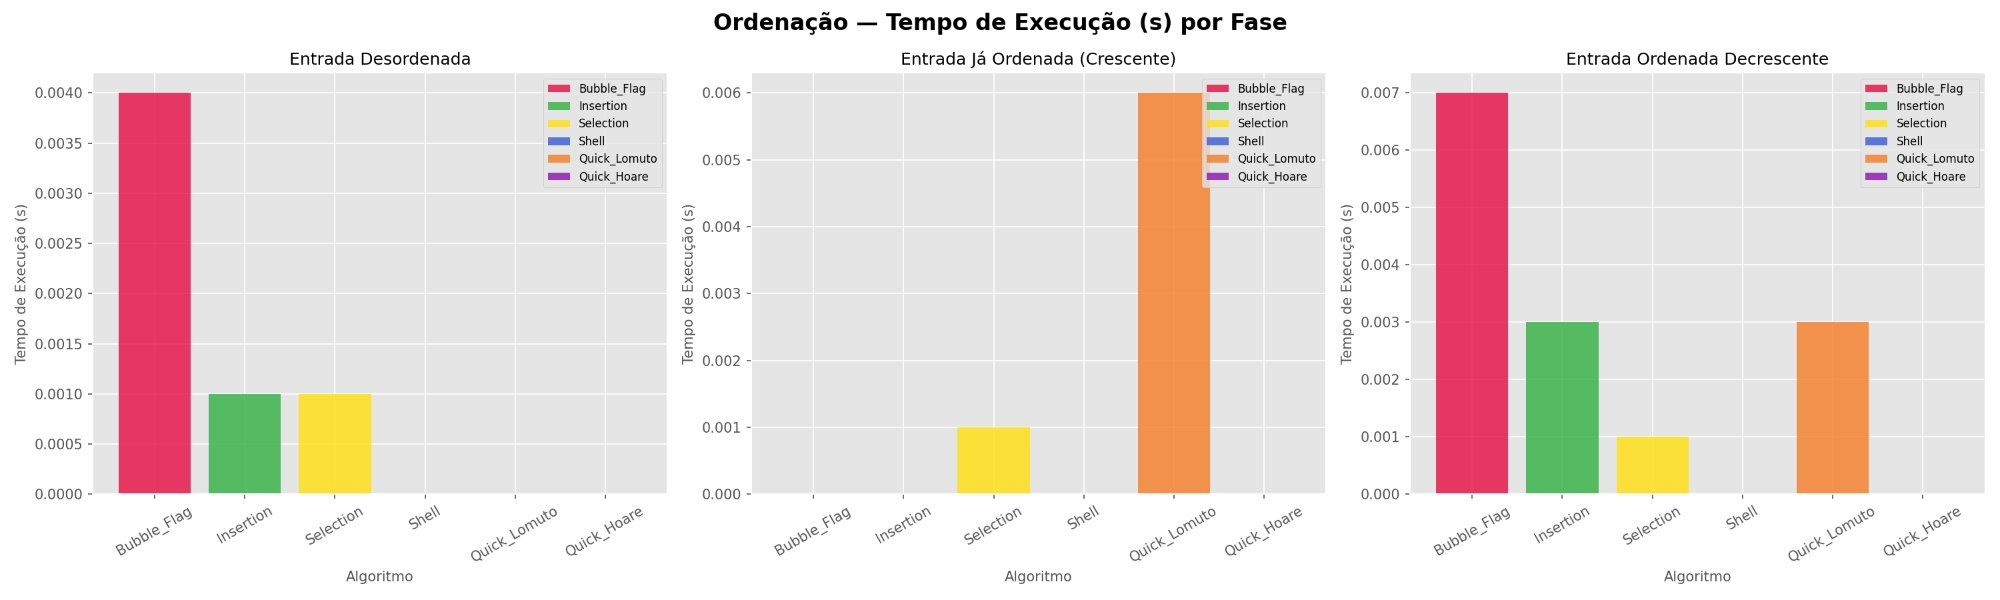
\includegraphics[width=\textwidth]{ord_tempos.png}
  \caption{Tempo de execução (s) por algoritmo nos três cenários de entrada (310 registros).}
  \label{fig:ord_tempo}
\end{figure}

\subsection{Algoritmos de Busca}

A Tabela~\ref{tab:busca_sequencial} apresenta os resultados da busca sequencial nos três estados dos dados para os três alvos selecionados.

\begin{table}[H]
\centering
\caption{Busca Sequencial --- comparações para cada alvo e estado dos dados.}
\label{tab:busca_sequencial}
\begin{tabular}{llrr}
\toprule
\textbf{Alvo} & \textbf{Estado dos dados} & \textbf{Comparações} & \textbf{Encontrado} \\
\midrule
63027 & Desordenado           &   1 & Sim \\
66804 & Desordenado           & 156 & Sim \\
33841 & Desordenado           & 310 & Sim \\
63027 & Ordenado Crescente    & 173 & Sim \\
66804 & Ordenado Crescente    & 199 & Sim \\
33841 & Ordenado Crescente    &  10 & Sim \\
63027 & Ordenado Decrescente  & 138 & Sim \\
66804 & Ordenado Decrescente  & 112 & Sim \\
33841 & Ordenado Decrescente  & 301 & Sim \\
\bottomrule
\end{tabular}
\end{table}

A Tabela~\ref{tab:busca_comparativa} compara diretamente a busca sequencial e a busca binária sobre dados ordenados em ordem crescente.

\begin{table}[H]
\centering
\caption{Busca Sequencial \textit{vs.} Busca Binária --- dados ordenados em ordem crescente.}
\label{tab:busca_comparativa}
\begin{tabular}{lrr}
\toprule
\textbf{Alvo} & \textbf{Sequencial (comparações)} & \textbf{Binária (comparações)} \\
\midrule
63027 & 173 & 9 \\
66804 & 199 & 8 \\
33841 &  10 & 8 \\
\bottomrule
\end{tabular}
\end{table}

A Figura~\ref{fig:busca_comp} ilustra graficamente esta diferença. À esquerda, a variação da busca sequencial nos três estados dos dados (média de 156 comparações no desordenado, 127 no crescente e 184 no decrescente). À direita, a comparação direta entre busca binária (média 8,3 comparações) e sequencial (média 127,3) sobre dados ordenados crescentes --- uma redução de \textbf{93,5\%} no número médio de verificações.

\begin{figure}[H]
  \centering
  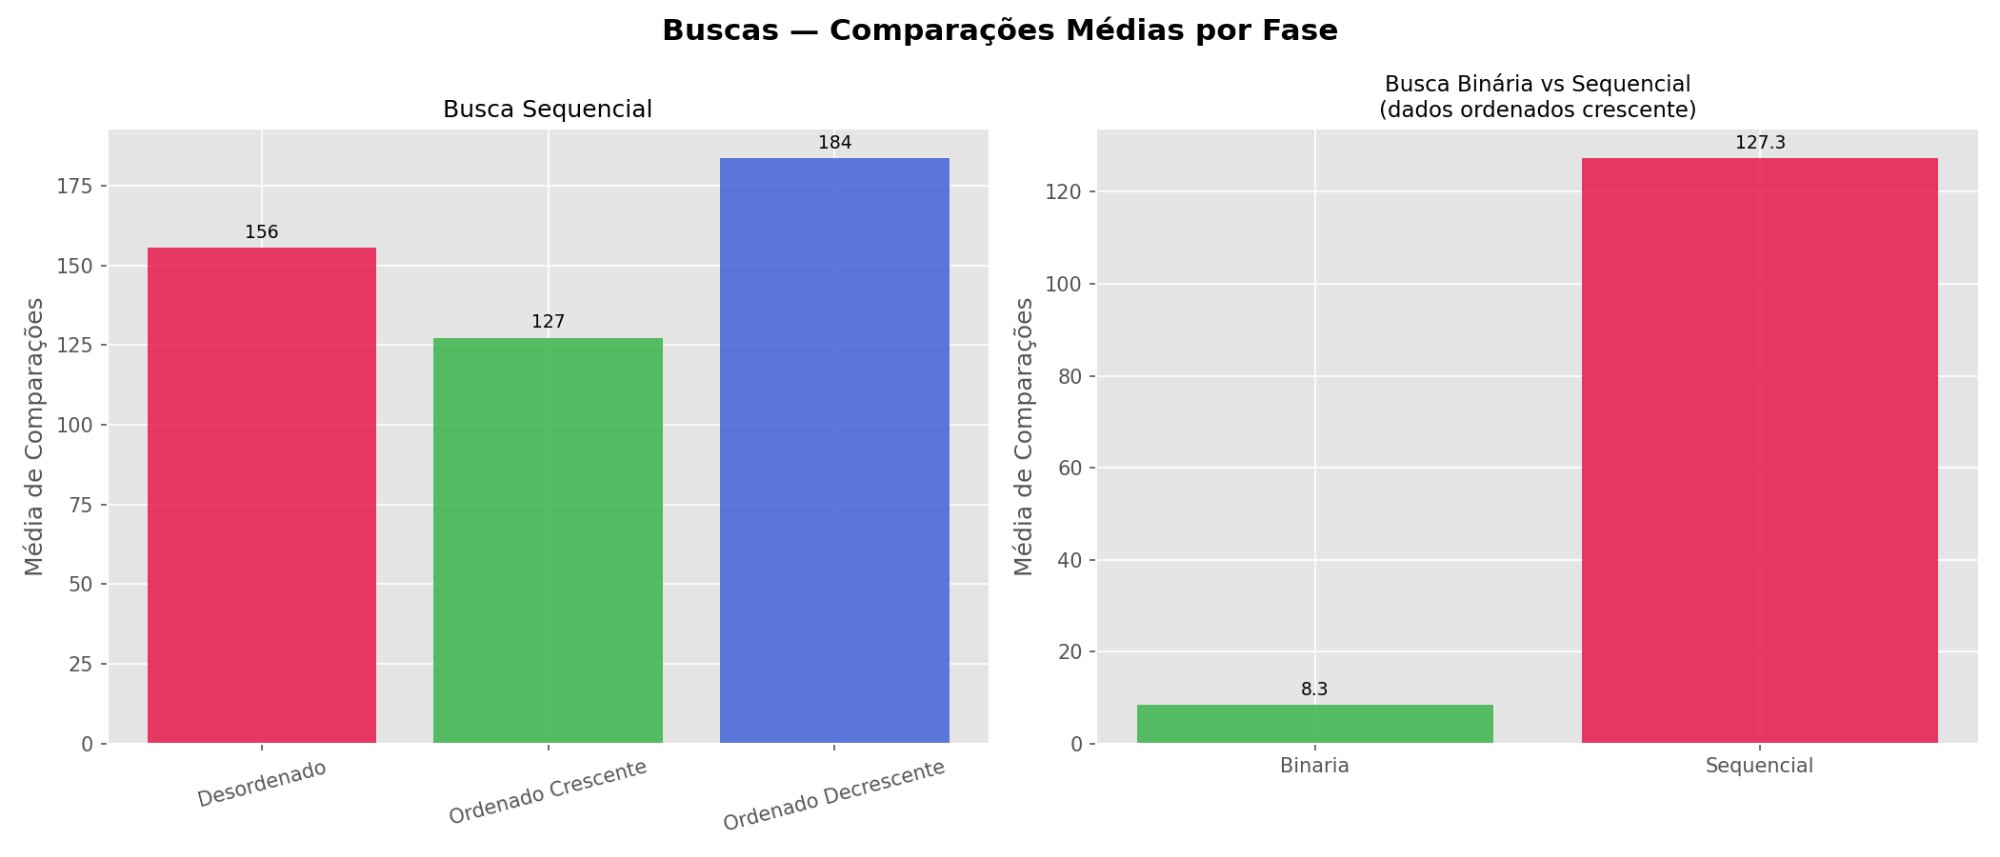
\includegraphics[width=\textwidth]{busca_comparacoes.png}
  \caption{Comparações médias da busca sequencial por fase (esq.) e comparação entre busca binária e sequencial sobre dados ordenados (dir.).}
  \label{fig:busca_comp}
\end{figure}

A Figura~\ref{fig:busca_tempo} registra os tempos de execução das buscas. Como o dataset possui apenas 310 registros, todos os tempos ficaram abaixo do limiar de resolução do \texttt{clock()}, registrando 0,000~s. Isso reforça que a análise de desempenho para conjuntos pequenos deve se basear principalmente no número de comparações --- a métrica independente de hardware e relógio.

\begin{figure}[H]
  \centering
  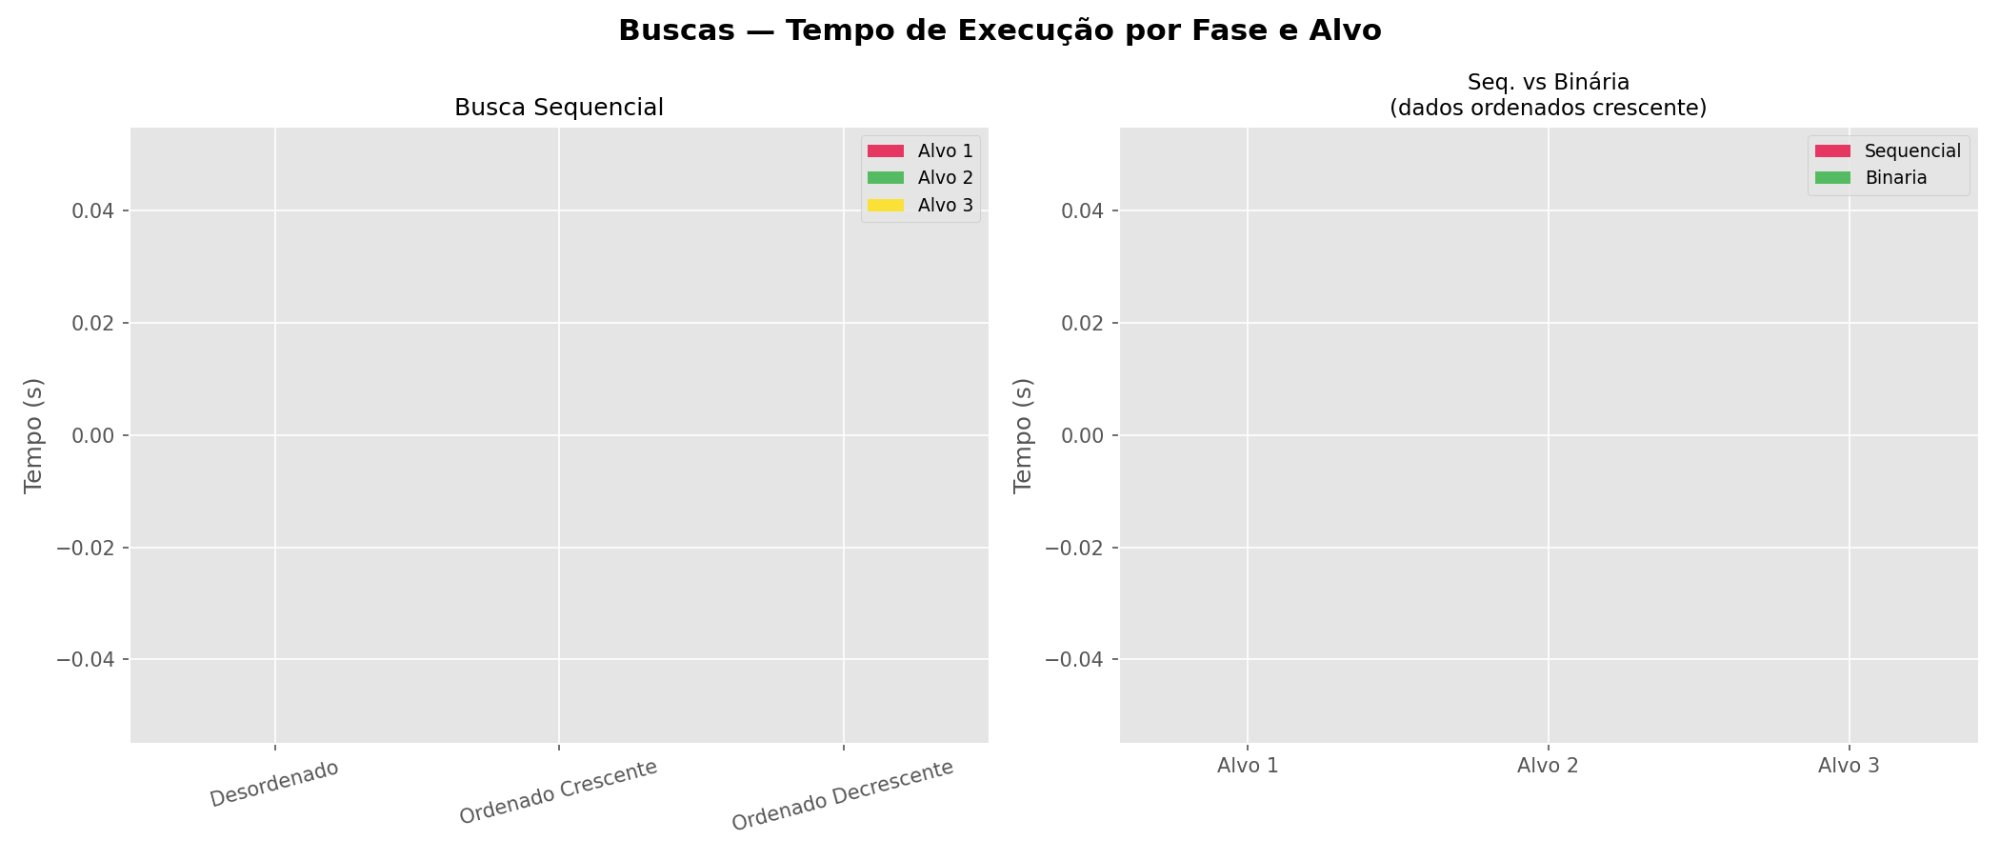
\includegraphics[width=\textwidth]{busca_tempo.png}
  \caption{Tempo de execução (s) das buscas por fase e alvo. Todos os valores ficaram abaixo da resolução do relógio de CPU utilizado.}
  \label{fig:busca_tempo}
\end{figure}

% -----------------------------------------------------------------------
\section{Análise Crítica}
\label{sec:analise}

\subsection{Comportamento dos Algoritmos de Ordenação}

\textbf{Bubble Sort com Flag} demonstrou seu comportamento bifurcado de forma clara: no cenário de dados já ordenados realizou apenas 309 comparações e zero trocas, confirmando a eficácia da flag de parada. No entanto, com dados desordenados ou invertidos acumulou respectivamente 47.859 e 47.895 comparações, além de 25.242 e 47.895 trocas. A elevada quantidade de trocas no pior caso ocorre porque cada elemento precisa "borbulhar" por toda a extensão do vetor até sua posição final.

\textbf{Insertion Sort} apresentou desempenho superior ao Bubble Sort no cenário desordenado, com 25.547 comparações (47\% menos) para a mesma quantidade de trocas (25.242). Isso ocorre porque, ao encontrar a posição correta de inserção, ele para antecipadamente --- não reinicia do início como o Bubble. No pior caso (ordem inversa), ambos convergiram para o mesmo custo.

\textbf{Selection Sort} exibiu o comportamento mais uniforme: 47.895 comparações em todos os cenários, porém com número mínimo de trocas --- apenas 306 no cenário desordenado e 155 no inverso. Essa característica o torna interessante quando o custo de movimentação física na memória é elevado, mas sua incapacidade de se beneficiar de dados parcialmente ordenados o torna inadequado como algoritmo geral.

\textbf{Shell Sort} demonstrou salto qualitativo expressivo: apenas 3.639 comparações e 1.640 trocas no cenário desordenado, tempo imesurável com a resolução do clock utilizado. A sequência de gaps reduziu drasticamente o deslocamento médio de cada elemento.

\textbf{Quick Sort Lomuto} foi o algoritmo com menor número de comparações no cenário desordenado (3.174), porém revelou sua vulnerabilidade ao dado já ordenado: 47.895 comparações e 48.204 trocas --- degeneração para $O(n^2)$ clássica, visível na Figura~\ref{fig:ord_comp} e na Figura~\ref{fig:ord_trocas}. Com o pivô sendo sempre o último elemento de um subvetor já ordenado, uma das partições fica vazia e a recursão se degenera em profundidade $n$.

\textbf{Quick Sort Hoare} demonstrou robustez nos três cenários: 4.245 comparações no desordenado, 48.513 no ordenado crescente (muitas comparações mas zero trocas), e 48.668 no decrescente com apenas 155 trocas. Sua estratégia de dois ponteiros convergentes cria um comportamento mais equilibrado e resistente ao pior caso do Lomuto.

\subsection{Impacto da Disposição Original dos Dados}

A disposição dos dados no arquivo CSV original (desordenados) mostrou ser o cenário mais representativo de produção. A diferença entre o Quick Sort Lomuto (3.174 comparações) e o Bubble Sort (47.859 comparações) neste cenário corresponde a uma razão de \textbf{15:1}. Em escala de 310 registros essa diferença é imperceptível ao usuário; porém, projetando para 310.000 registros (fator $10^3$), o Bubble Sort executaria aproximadamente $4,8 \times 10^{10}$ operações contra $\sim 5,2 \times 10^6$ do Quick Sort --- uma diferença de quatro ordens de grandeza.

\subsection{Busca Sequencial \textit{vs.} Busca Binária}

Como evidenciado na Figura~\ref{fig:busca_comp}, a busca binária reduziu o número máximo de comparações para apenas 9 (alvo 63027) e 8 (alvos 66804 e 33841), confirmando o limite teórico $\lceil \log_2 310 \rceil = 9$ iterações. A comparação mais expressiva ocorre com o alvo 33841: a busca sequencial em dados desordenados precisou de 310 comparações (100\% do vetor), enquanto a busca binária localizou o mesmo elemento em 8 comparações --- uma redução de \textbf{97,4\%}. Estes dados justificam plenamente o custo da ordenação prévia quando o sistema realizará múltiplas consultas sobre o mesmo conjunto de dados.

% -----------------------------------------------------------------------
\section{Conclusões}
\label{sec:conclusao}

Este trabalho analisou empiricamente seis algoritmos de ordenação e dois de busca sobre um dataset biomédico real de 310 registros da coluna vertebral. Os resultados obtidos corroboram as previsões teóricas e permitem formular recomendações práticas objetivas.

Para um sistema de produção que manipule dados desta natureza --- registros médicos numéricos que chegam desordenados e precisam ser consultados frequentemente --- a combinação recomendada pela equipe é:

\begin{enumerate}
  \item \textbf{Quick Sort Hoare} como algoritmo de ordenação principal: menor número de trocas físicas (606) no cenário desordenado, comportamento robusto nos três cenários e ausência da degeneração $O(n^2)$ que penalizou o Lomuto com dados já ordenados.
  \item \textbf{Shell Sort} como alternativa para ambientes com restrição de pilha de recursão (sistemas embarcados), dado seu excelente desempenho (3.639 comparações) sem recursão.
  \item \textbf{Busca Binária} como único método de consulta após a ordenação inicial: a redução de até 97,4\% no número de comparações em relação à busca sequencial é determinante para a escalabilidade do sistema.
  \item \textbf{Evitar Bubble Sort} em dados desordenados de médio/grande porte, reservando-o apenas para re-ordenações incrementais de datasets quase ordenados onde seu custo linear se manifesta.
\end{enumerate}

Como trabalhos futuros, recomenda-se expandir a análise para datasets com 50.000 ou mais registros para que as curvas de crescimento assintótico se manifestem de forma mais pronunciada, e investigar estratégias de pivô adaptativas no Quick Sort (como mediana de três elementos) para mitigar o pior caso na variante Lomuto.

% -----------------------------------------------------------------------
\bibliographystyle{sbc}
\begin{thebibliography}{9}

\bibitem{cormen2002}
CORMEN, T. H.; LEISERSON, C. E.; RIVEST, R. L.; STEIN, C.
\textbf{Introduction to Algorithms}. 2. ed. Cambridge: MIT Press, 2002.

\bibitem{ziviani2005}
ZIVIANI, N.
\textbf{Projeto de Algoritmos com Implementações em Pascal e C}. 2. ed.
Belo Horizonte: Editora Pioneira Thomson, 2005.

\bibitem{sedgewick1996}
SEDGEWICK, R.
\textbf{Algorithms in C: Parts 1--4 -- Fundamentals, Data Structures, Sorting, Searching}. 3. ed.
Reading: Addison-Wesley, 1998.

\bibitem{medina2005}
MEDINA, M.; FERTING, C.
\textbf{Algoritmos e Programação: Teoria e Prática}. 1. ed.
São Paulo: Novatec, 2005.

\bibitem{uci_spine}
BERTHONNAUD, E. et al.
\textbf{Vertebral Column Data Set}.
UCI Machine Learning Repository, 2011.
Disponível em: \url{https://archive.ics.uci.edu/ml/datasets/Vertebral+Column}.
Acesso em: abr. 2026.

\bibitem{azevedo2015}
AZEVEDO, R. C. de.
\textbf{Análise dos Algoritmos de Ordenação: buscando a eficiência em sistemas de supermercados}.
Relatório Final PIBIC/PAIC 2015--2016.
Manaus: Universidade Federal do Amazonas, 2016.

\bibitem{taroco2014}
TARÔCO, J.; SANTOS, E.
\textbf{Uma Comparação de Algoritmos de Ordenação}.
Minas Gerais, 2014.

\end{thebibliography}

\end{document}
